\documentclass{article}
\usepackage[utf8]{inputenc}
\usepackage{amsmath}
\usepackage{theorem}
\usepackage{algorithm,algorithmic}
\hyphenation{PageRank}
\hyphenation{PageRanks}
\usepackage{tikz}
\usepackage{titlesec}
\usepackage{amsmath}
\usepackage{caption}
\usepackage{graphicx}
\usepackage{natbib}
\usepackage{graphicx}
\usepackage{svg}

\usepackage{algorithm}
\usepackage{algpseudocode}

\captionsetup{labelfont={bf}}

\title{Bayesian Computing}
\author{Ashutosh Singh}
\date{June 2021}

\begin{document}

\maketitle

\section{Introduction}
Vector quantization or clustering is a very important topic in Machine Learning. Unsupervised clustering techniques are use to group people with similar symptoms, group similar queries on a forum or in the context of this report grouping users based on their behaviour on a website.

Goal is to utilize Intrinsic Dimension based methodology HIDALGO to find clusters of users. To this end we chose to use the intRinsic R-package which provides very good set of of APIs and methods to run HIDALGO and analyze its results


\section{Dataset}
The dataset consists of events of each user along with timestamp of the event. Dataset sample

\begin{table}[ht]
      \centering
      \begin{tabular}{|c | c | c | c | c|}
             \hline
             event\_date & event\_timestamp & event\_name & user\_id\\
             \hline
             \hline
             20210425 & 1.619378e+15 & login & APP-055rKogJet...\\
             \hline
             20210425 & 1.619378e+15 & user\_engagement& APP-055rKog...\\
             \hline
      \end{tabular}
    \caption{A sample of original dataset. Complete dataset has 2699 observations like the two shown above across 4 variables}
    \label{tab:table-name}
 \end{table}
 
\subsubsection{Events}
Events are the manifestation of user's browsing behaviour on the website.
There a total of 25 unique events.

\subsubsection{Users}
Users of the website. There are a total of 136 users in the dataset. Out of which 108 have unique behaviour.

\section{Segmentation with Hidalgo}

\subsection{Transforming the dataset}
This structure of dataset is not suitable for clustering users. Performing the following transformation steps - 
\begin{enumerate}
    \item Represent each user as a 25-D vector
    \item Each dimension in the vector represents a unique event.
    \item The value of the event-index for user vector is the number of times user triggered this event
    \item For all the events a user doesn't trigger that user never visits the value is 0(zero)
\end{enumerate}

After following the above steps the dataset looks like - 

\begin{figure}[H]
\centering
  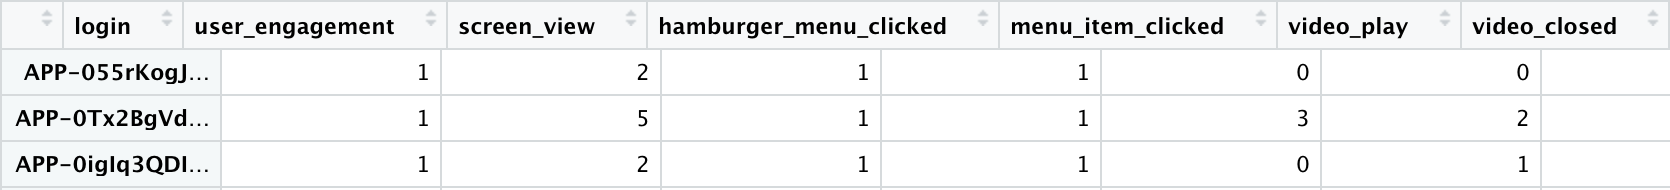
\includegraphics[width=1\textwidth]{Trandformed.png}
  \caption{Transformed dataset. 136x25 matrix. 136 users and 25 unique events. Here only 6 events are shown.}
\label{fig}
\end{figure}

\subsection{Running Hidalgo}
Running the Hidalgo algorithm from intRinsic R-package on the transformed data following results are observed.

\begin{figure}[H]
  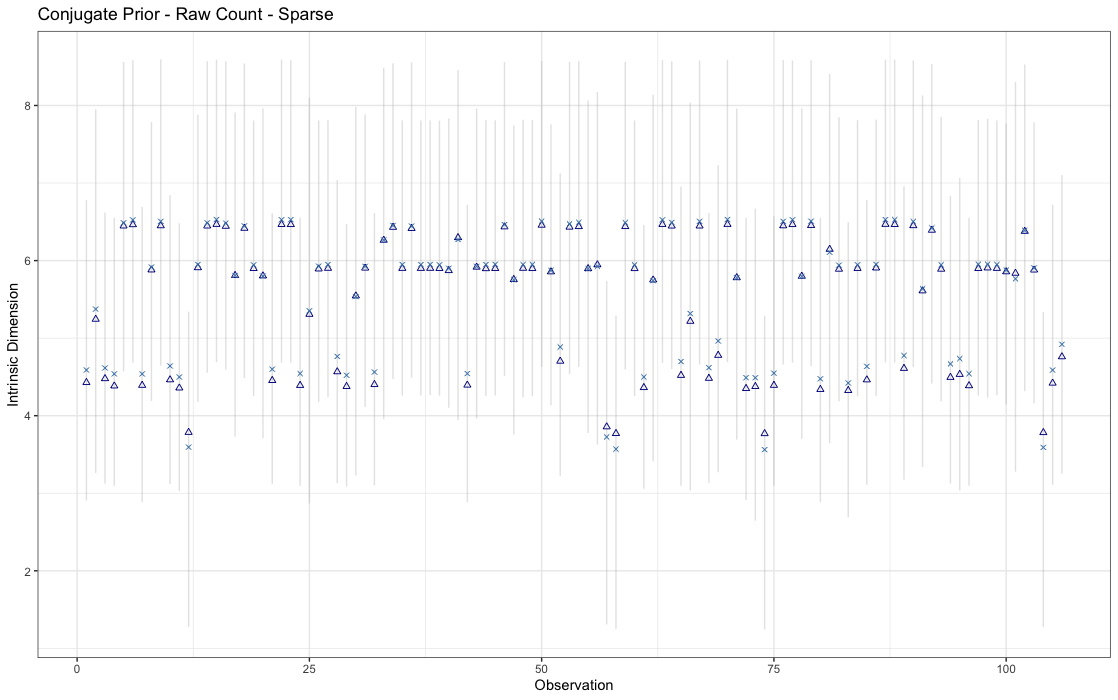
\includegraphics[width=1.3\textwidth]{RawCount-ConjugatePrior-Sparse.png}
  \caption{Plot of users(X-axis) and ID(Y-axis) with a Conjugate Prior. Burn-in=2500 and nSim=5000. Triangles are median values and crosses are mean values of ID. The grey vertical lines represent a 90\% credible interval}
\label{fig}
\end{figure}

\subsection{Inducing state dependence}
The clusters look good and the results from above mentioned transformation and Hidalgo are quite impressive.

But there are certain problems with the above approach.
It doesn't take user's previous state into account when considering his score for an event.

\subsubsection{Checking for Markov Property}
The above raw-scores just measure how many times a user triggered the event. 

So with this in mind I tried to look for Markov Property.
These are the steps I followed:
\begin{enumerate}
    \item Take the entire event\_name column from the original dataset i.e. a column vector of size 2699.
    \item Used "verifyMarkovProperty" method of the "markovchain" package to see the results
    \item Results: 
    Chi - square statistic is: 1571.218 \\
    Degrees of freedom are: 224 \\
    And corresponding p-value is: 0 
    \item As we can see the p-value is really small. Hence we can reject ${H_0}$ that Markov Property exists
\end{enumerate}

This approach seemed to be the best approach. But after getting these results, I realized the mistake that was made.
Each user accesses the markov chain independently. So taking the entire event column is not the right way

\subsubsection{Making a transition matrix}
The entire event column should not be used to verify Markov Property.

To create a transition matrix for transitions between events the following steps were taken:

\begin{enumerate}
    \item Use chain of events visited by each user to make a transition count matrix
    \item The chain ends with each user and is restarted for the next user.
    \item Code iterates for each user from the 2nd event he triggered till the last event.
    \item Divide each element in row by the sum of all elements in that row to get transition probabilities.
\end{enumerate}

\subsubsection{Making a Markov Chain}
Now that the transition matrix is ready I use the markovchain package to create our Markov chain.

And this time I got a favourable result, the Markov Chain is Irreducible and Aperiodic and hence there is unique limiting distribution.

I store this transition matrix and limiting distribution and put them to use in the subsequent sections.


\subsubsection{Transforming the data}
With the transition matrix I obtained I modified the Data transformation steps mentioned in Section 3.1 to induce state dependence.

Now To represent each user as a 25-D vector, I follow the steps mentioned below - 
\begin{enumerate}
    \item Get the sequence of events for the user.
    \item Give the first event of each user a score of 1
    \item Iterate over the sequence of steps for the user from 2nd event and use transition\_matrix[i-1, i] as the score for i-th event.
    \item Every event the user doesn't visit he gets a 0(zero) score.
\end{enumerate}

This method improves upon the previous data transformation process by inducing a state dependence.
For example a user triggering event-2 after event-1 would be an exact copy of user triggering event-1 after event-2; if we go with the transformation steps in section 3.1.

But here this is not true. We get different vectors for bot of these hypothetical users

I think it's a very nice property

\subsubsection{Running Hidalgo with new data}
\begin{figure}[H]
  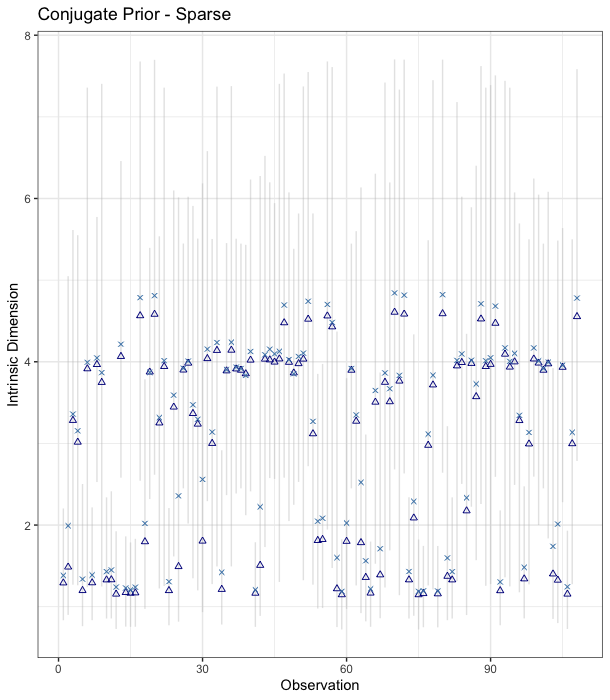
\includegraphics[width=1.3\textwidth]{SparseTransition-ConjugatePrior.png}
  \caption{Plot of users(X-axis) and ID(Y-axis) with a Conjugate Prior. Burn-in=2500 and nSim=5000. Triangles are median values and crosses are mean values of ID. The grey vertical lines represent a 90\% credible interval}
\label{fig}
\end{figure}

{Even without a manual check we can see that the credible intervals are more disconnected for observations in different ID levels}.

\subsubsection{One final trial}
The above data transformation brings the previous state into play when giving the score for current state; but it still leaves the unvisited events with a zero score.

Since we already have a stationary distribution I decided to replace 0 for an event in a user vector with its limiting distribution probability.

And ran this modified data through Hidalgo. The previous data matrix was sparse but new modified matrix is dense hence the title of the chart.

\begin{figure}[H]
  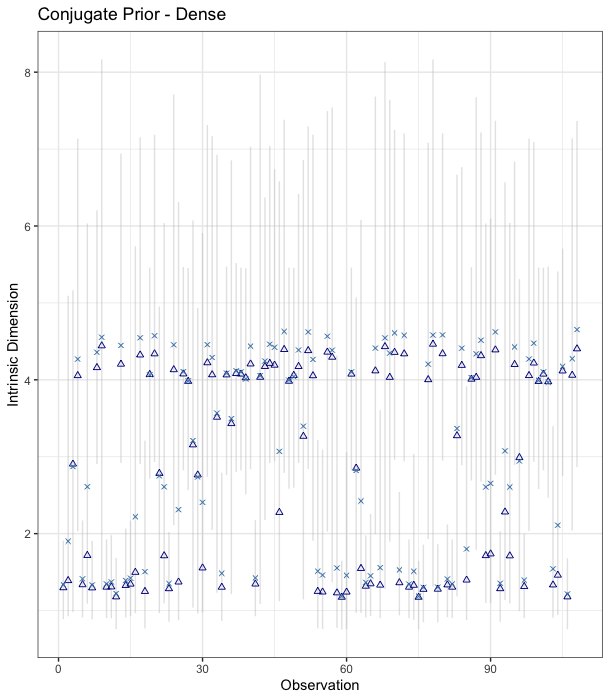
\includegraphics[width=1.3\textwidth]{DenseTransition-ConjugatePrior.png}
  \caption{Plot of users(X-axis) and ID(Y-axis) with a Conjugate Prior. Burn-in=2500 and nSim=5000. Triangles are median values and crosses are mean values of ID. The grey vertical lines represent a 90\% credible interval. These results are for Dense Matrix we just obtained}
\label{fig}
\end{figure}

\section{Analysis of Results}
Now we get to the part where we make comparisions on all Hidalgo outputs.
\begin{enumerate}
    \item Raw-Count: Using this term to represent the first run with results in section 3.2
    \item Sparse-Transition: For the run where use transition probabilities as scores. Section 3.3.1 - 3.3.5
    \item Dense-Transition: For the third last trial . Section 3.3.6 
\end{enumerate}

\subsection{Visual observations}
As we can see from Figure-2, Figure-3 and Figure 4 for Raw-Count, Sparse-Transition and Dense-Transition, the credible interval lines(the vertical grey lines) become more visibly separate from each other as we go from Raw-Count to Dense-Transition

This implies that model is becoming more confident in segregating the users.


\subsection{Comparing Optimal Clusters}
I will now only compare Dense-Transition and Sparse-Transition.

I use Hidalgo\_coclustering\_matrix method from R-package. The results also confirm what we saw visually.

I most cases both these iterations give same result. The results for level 3 are exactly same for both methods.

However these methods predict don't agree with each other in the following cases


\begin{figure}[H]
  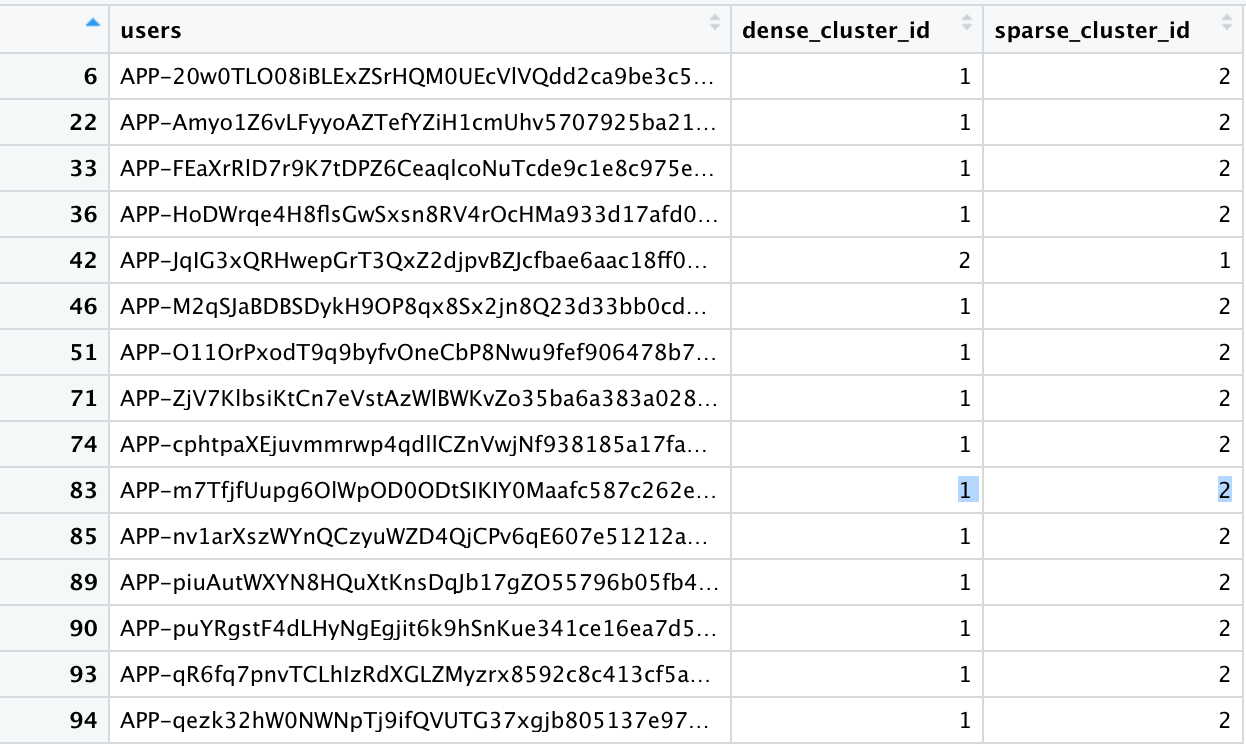
\includegraphics[width=1.3\textwidth]{Diff-Between-Desne-Sparse.png}
  \caption{Users for which we get different results from Dense-Transition and Sparse-Transition}
\label{fig}
\end{figure}


\subsection{Comparing Discriminatory Power}
To support the visual observation that Dense-Transition is better at discriminating the clusters as visible from 90\% credible intervals.

For this purpose we need to inspect the posterior co-clustering matrix.

A method that takes in each user which is classified under different clusters and uses co-clustering matrices from Dense-Transition and Sparse-Transition to get the posterior scores of user with other users in same cluster and users in other clusters.
Compute mean of absolute value of diff between above two scores.

The method for which this mean is higher should indicate higher confidence.

Out of the 15 incorrectly classified users we get 8 users having these mean values higher for Dense-Transition than for Sparse-Transition

But this is not a very dependable method or accurate method. Since the overall scale of both runs i.e. Dense-Transition and Sparse-Transition might be different.

I leave finetuning this method for future work.


\subsection{Manual analysis}

To further check the performance of Dense-Transition and Sparse-Transition, I did a manual check on the cluster they have the most different results for - Cluster-2.
Adding the results in cluster\_2\_users\_dense.csv and cluster\_2\_users\_sparse.csv



\section{Future Work}
\subsection{Using different Distance metric}
We can try using a different distance metric than Hidalgo uses right now. Instead of Euclidean Distance we can try using Cosine-Similarity and see the results.
Instead of spatial-distance Cosine-Similarity focusses on orientation.

\subsection{Induce a time dependence}
In addition to having dependence on previous event we can also think towards adding a time dependence.

Since the time between two events is not scaled we will need to handle that as well. We can look into recently introduced time-embedding methods for that.

\subsection{Sophisticated Discriminatory Power measures}
Improve the method in section 4.3 or develop new methods to measure this.

\subsection{Human annotation}
I did a very basic experiment with cluster 2 as mentioned in section 4.4. But to get a more clear idea on algorithm's behaviour we need to do more human annotation


% \subsubsection{Variables}
% \begin{enumerate}
%     \item \texttt{dense\_cluster\_id} - Cluster id as predicted by Dense-Transition
%     \item \texttt{sparse\_cluster\_id} - Cluster id as predicted by Sparse-Transition
%     \item \texttt{dense\_psm} - Co-clustering matrix for Dense-Transition
%     \item \texttt{sparse\_psm} - Co-clustering matrix for Sparse-Transition
%     \item \texttt{result} - Dataframe with three columns; users, dense\_cluster\_ids and sparse\_cluster\_ids
% \end{enumerate}

% \texttt

% \subsubsection{Algorithm}
% \begin{algorithm}
%   \caption{Basic scoring mechanism}
%       \For{each \texttt{user} classified under diff cluster}
%       \\
%       {\# For Dense-Transition}\\
%       \State {Filter \texttt{result} dataframe to remove \texttt{user} to get \texttt{temp}}
%       \State {Get users from \texttt{temp} with dense\_cluster\_ids equal to \texttt{dense\_cluster\_id} in \texttt{dense\_users}}
%       \State {Get users from \texttt{temp} with dense\_cluster\_ids equal to \texttt{sparse\_cluster\_id} in \texttt{sparse\_users}}
%       \State {Get top scorers from  \texttt{dense\_psm}[\texttt{user}, \texttt{dense\_users}]}
%       \State {Get top scorers from  \texttt{dense\_psm}[\texttt{user}, \texttt{sparse\_users}]}
%       \State {Calculate mean of absolute values of differences of above two scores as \texttt{dense_mean}}
%       \\
%       {\# Repeat the same steps for Sparse-Transition to get \texttt{sparse_mean}}\\
      
%       \State{Compare \texttt{sparse_mean} and \texttt{dense_mean}}
%       \EndFor
% \end{algorithm}

\section{Results and Files}
\subsection{Code}
\begin{enumerate}
    \item pr.R - File with Dense-Transition and Sparse-Transition Methods code
    \item raw\_count.R - File with Raw-Count method code
\end{enumerate}


\subsection{Data}
\begin{enumerate}
    \item results-20210426-141638.csv - Original data file
    \item user\_rows.R - Data file with users as rows and their events in columns. Each row has different lengths.
\end{enumerate}


\subsection{Results}
All the files related to this section are in `results` directory
\begin{enumerate}
    \item cluster\_2\_users\_dense.csv - Results of manual analysis of cluster 2
    \item cluster\_2\_users\_sparse.csv - - Results of manual analysis of cluster 2 Sparse-Transition
    \item RawCount-ConjugatePrior-Sparse.png - Hidalgo results Raw-Count
    \item DenseTransition-ConjugatePrior.png - Hidalgo results Dense-Transition
    \item SparseTransition-ConjugatePrior.png - Hidalgo results Sparse-Transition
\end{enumerate}





\end{document}

